\documentclass[12pt]{article}
\usepackage{indentfirst}
\usepackage{enumitem}
\usepackage{amsmath}
\setlength{\jot}{2ex}
\usepackage{mathrsfs}
\usepackage{graphicx}
\usepackage{wrapfig}
\usepackage{booktabs}
\usepackage[letterpaper, margin=1in]{geometry}
\usepackage{fancyhdr}
\pagestyle{fancy}
\fancyhead[R]{Chapter 2}
\fancyfoot[C]{\thepage}
\renewcommand{\headrulewidth}{1pt}
\renewcommand{\footrulewidth}{1pt}
\usepackage [autostyle, english = american]{csquotes}
\MakeOuterQuote{"}
\renewcommand{\baselinestretch}{1.0}
\newcommand{\objects}[2]{%
  \leavevmode\vbox{\hbox{#1}\nointerlineskip\hbox{#2}}%
}
\begin{document}
    \section*{Introduction}
    \par Computer design is set to achieve a common goal, find a language that
    makes it easy to build the hardware and the compiler while maximizing
    performance and minimizing cost and energy.
    \par The "simplicity of the equipment" is a valuable part of designing a
    machine, as the more simplistic the instructions to be interpreted, the
    better the overall performance gains will be. Section 2.15 shows how the
    examples will change with object-oriented languages.
    \section*{Operations of the Computer Hardware}
    \par Notation for performing arithmetic in RISC-V assembly language:
    \[
        \text{add a, b, c}
    \]
    This gives the computer instructions to add the two variables b and c
    and store the value of that in the variable a. This notation can only use
    three variables at a time, due to the concept of simplicity. The less
    variables the computer has to deal with at a time, the faster the operation
    will be and for this reason, arithmetic is done on multiple lines.
    \par For example, take the equation f = a + b + c + d, this would have to
    be written as,
    \begin{align*}
        &\text{add f, a, b}\qquad //\ \text{The sum of a and b is stored in f} \\
        &\text{add f, f, c}\qquad //\ \text{The sum of a, b, and c is stored in f} \\
        &\text{add f, f, d}\qquad //\ \text{The sum of a, b, c, and d is stored in f}
    \end{align*}
    \par This gives the sum of the four variables and stores its value into f. The
    two slash marks indicate a comment and explain what is happening at each of
    the steps.
    \begin{figure}[h]
        \centering
        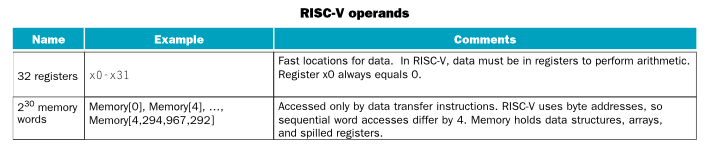
\includegraphics[width=1\textwidth]{RISC-V operands.png}
    \end{figure}
    \par This table explains what the "variables" in the examples are supposed
    to be. According to the standards of RISC-V, in order to perform arithmetic
    on some data, the data must be in the CPU registers. This makes accessing
    them easier than parsing through memory, making computations faster and
    therefore improving the overall performance of the machine. There are 32
    32-bit registers, ranging from x0 to x31. The number of operands for
    addition is 3, the two numbers being added and a place to put the sum.
    \newpage
    \begin{figure}[h]
        \centering
        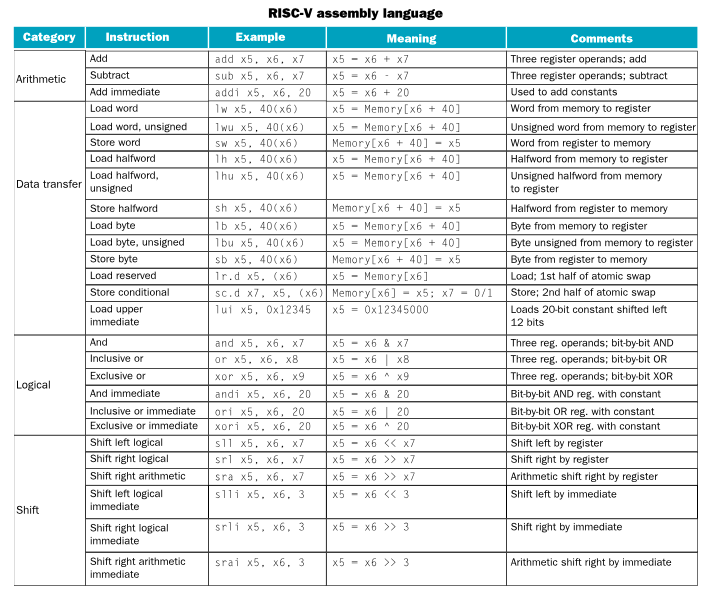
\includegraphics[width=1\textwidth]{RISC-V commands.png}
    \end{figure}
    \par These are the list of built in functions that can be used by the
    assembly language to give instructions. It can be seen that many of these
    commands have only three operands. This is to serve the purpose of
    simplicity. \textbf{Design Principle 1: Simplicity favors regularity.}
    \subsubsection*{Example:}
    \par Take for example these operations written in high-level languages such
    as C,
    \begin{align*}
        & \text{a = b + c;} \\
        & \text{d = a -- e;}
    \end{align*}
    \par The compiler will translate this from the C language to RISC-V and
    create the assembly instructions,
    \begin{align*}
        & \text{add a, b, c} \\
        & \text{sub d, a, e}
    \end{align*}
    \subsubsection*{Example:}
    \par Take the equation f = (g + h) - (i + j); what would the C compiler
    produce? There are multiple variables here and we know that the assembly
    language can only make use of three at a time.
    \begin{align*}
        & \text{add t0, g, h}\qquad //\ \text{Temp variable t0 takes on the value of g + h} \\
        & \text{add t1, i, j}\qquad //\ \text{Temp variable t1 takes on the value of i + j} \\
        & \text{sub f, t0, t1}\qquad //\ \text{f takes on the value of (g + h) - (i + j)}
    \end{align*}
    \par It can be seen here that this process takes three lines of code where
    as in the high level language the equation was merely one line. First it
    adds the two variables that need adding together, g and h, and i and j, and
    then takes the values of these sums and subtracts them to get the desired
    output for f.
    \section*{Operands of the Computer Hardware}
    \subsection*{Register Operands}
    \par The operands in assembly languages are restricted in that they must
    come from a specified place. These places are known as \textit{registers}
    and the reason for this, as stated before, is for performance enhancement.
    The closer the objects are to the CPU and the easier they can be accessed,
    the faster the program will be able to run.
    \par \textbf{Word} -- corresponds to a unit of access in a computer, a group
    of 32 bits. RV32 refers to the size of a RISC-V register which is 32 bits.
    \par \textbf{Doubleword} -- corresponds to a unit of access in a computer, a group
    of 64 bits. RV64 refers to the size of a RISC-V register which is 64 bits.
    \par Most computers use 32 registers and the RV32 architecture will be most
    often used. In both cases, the restriction on the number of registers to 32
    is due to the principle that smaller is faster. \textbf{Design Principle 2:
    Smaller is faster.} A large number of registers may increase the clock cycle
    time since the signals inside the chip will have to travel a farther
    distance. The registers 0 through 31 are indicated with the letter x and the
    number of the register following.
    \par Taking the same example as before and fixing it so that it uses
    registers instead of arbitrary variables, let's say that f, g, h, i, and j
    are assigned to the registers x19, x20, x21, x22, and x23. We will also have
    to have two registers open to store the temporary values, let's call that x5
    and x6.
    \begin{align*}
        & \text{add x5, x20, x21}\qquad //\ \text{Register x5 takes on the value of g + h}  \\
        & \text{add x6, x22, x23}\qquad //\ \text{Register x6 takes on the value of i + j}  \\
        & \text{add x19, x5, x6}\qquad //\ \text{Register x19 takes on the value of (g + h) - (i + j)}
    \end{align*}
    \par This is the correct RISC-V assembly language code as it uses the
    registers to store and retrieve the values needed for calculation.
    \subsection*{Memory Operands}
    \par Programming languages can have simple single data elements, as shown
    in the examples above, but they also can have more complex data such as
    arrays and structures. How can these be represented in the assembly
    language?
    \par The processor can only hold a small amount of data in its registers,
    however, the computer memory has billions of data cells. Data structures for
    this reason are stored within the computer memory.
    \par Since arithmetic operations can only occur within the registers of the
    processor, there must be some method by which RISC-V can transfer data from
    memory to the registers.
    \par \textbf{Data Transfer Instruction} -- a command that moves data between
    the memory and the CPU registers.
    \par \textbf{Address} -- a value used to define the location of a specific
    data element within the memory array.
    \begin{figure}[h]
        \centering
        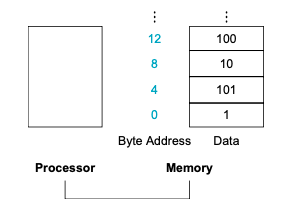
\includegraphics[width=0.4\textwidth]{Processor Memory Interaction.png}
    \end{figure}
    \par Memory can be thought of as a large single dimensional array, where the
    address is like a specific index of the array, starting from 0. From the
    picture above it can be seen that the data in index [2], which has a
    byte address of 8 in the memory, would be 10.
    \par The data transfer instruction is usually referred to as load. To
    load data into a register, the "load word" instruction would be used.
    \subsubsection*{Example:}
    \par Assume that there is an array A which consists of 100 words and is
    assigned to the register x22, and that the variables g and h are associated
    to the registers x20 and x21. If the code is C is g = h + A[8], what is the
    compiled code in RISC-V?
    \par Since one of the operands, A[8], resides in the memory, it must first
    be transferred to a register, for example register x9. This is done by the
    following notation,
    \[
        \text{lw x9, 32(x22)}\qquad //\ \text{Temp reg x9 takes value of A[8] from memory}
    \]
    \par Here, the word is being loaded into the register x9 and it is important
    to realize the notation that A[8] takes in the code. The notation for the
    array is defined as, \\ Byte Address(Array Register). The Byte
    Address can be determined by taking the desired index and multiplying it by
    4, and adding on the base Byte Address,
    \[
        \text{Byte Address = Index $\times$ 4 + Base Byte Address}
    \]
    \par This is where the 32 comes from in the notation. The Base Byte Address
    refers to the first Byte Address, and in this case, since it is 0, the Byte
    Address for A[8] will simply be, 8 $\times$ 4 = 32.
    \par Now that the data from memory is stored in a register, x9, the rest of
    the arithmetic can be carried through. The full code would be,
    \begin{align*}
        & \text{lw x9, 32(x22)}\qquad //\ \text{Loads A[8] into register x9} \\
        & \text{add x20, x21, x9}\qquad //\ \text{Places sum of h + A[8] into g}
    \end{align*}
    \par With that, the statement is completely compiled from C to RISC-V.
    \subsubsection*{Example:}
    \par Now, take the same example above, and instead of storing the value into
    g, store it into the array at index 12, A[12].
    \par Here, there is not much different from the previous problem other than
    the fact that now we need to store the value into memory as well. The first
    steps will be the same, except the addition will go to the temp register
    instead of one for the variable g.
    \begin{align*}
        & \text{lw x9, 32(x22)}\qquad //\ \text{Loads A[8] into register x9} \\
        & \text{add x9, x21, x9}\qquad //\ \text{Places sum of h + A[8] into register x9}
    \end{align*}
    \par The last thing to do is store the value of register x9 into A[12].
    Using the technique to define the operand for A[8], the same can be done for
    A[12], 12 $\times$ 4 = 48, \\ A[12] $\implies$ 48(x22). The value can then be
    stored using the "store word" instruction, sw. The full code would then be:
    \begin{align*}
        & \text{lw x9, 32(x22)}\qquad //\ \text{Loads A[8] into register x9} \\
        & \text{add x9, x21, x9}\qquad //\ \text{Places sum of h + A[8] into register x9} \\
        & \text{sw x9, 48(x22)}\qquad //\ \text{Places x9, h + A[8], into A[12]}
    \end{align*}
    \rule{\textwidth}{0.25pt} \\
    \par Many programs have more variables than the computer has registers and
    for this reason, the computer must move variables around between registers
    and memory. The most important variables are kept in the registers and the
    rest are stored in memory. The processes of keeping less frequently used
    variables in memory is called \textit{spilling registers}.
    \subsection*{Constant or Immediate Operands}
    \par In many cases, there will be a constant that is being used within a
    program and in fact, this is the most common case which means, it must be
    made as fast as possible. It would not make sense to load the constant into
    a register of its own just for operation, that would take too long instead,
    immediate operations are used.
    \par These operations are used in the case that there is a content which is
    easy to add on and does not require its own dedicated register. If say we
    are adding 4 to the contents of the register x22, the code would simply be,
    \[
        \text{addi x22, x22, 4}\qquad //\ \text{x22 = x22 + 4}
    \]
    \par By including constants as operands to arithmetic instructions, the
    operations are much faster and require less energy than if they were being
    loaded in from memory.
    \par The constant 0 has a specific role as it is used to simplify the
    instructions by offering useful variations. For example, a number can be
    negated by using the subtraction instruction with 0 as the first operand.
    For this reason RISC-V dedicates the first register, x0, to always equal 0.
    This is another example of making the common case fast.
    \section*{Representing Instructions in the Computer}
\end{document}
